\chapter{The First Appendix}
\label{app:A}

\begin{figure}[htbp]
    \centering
    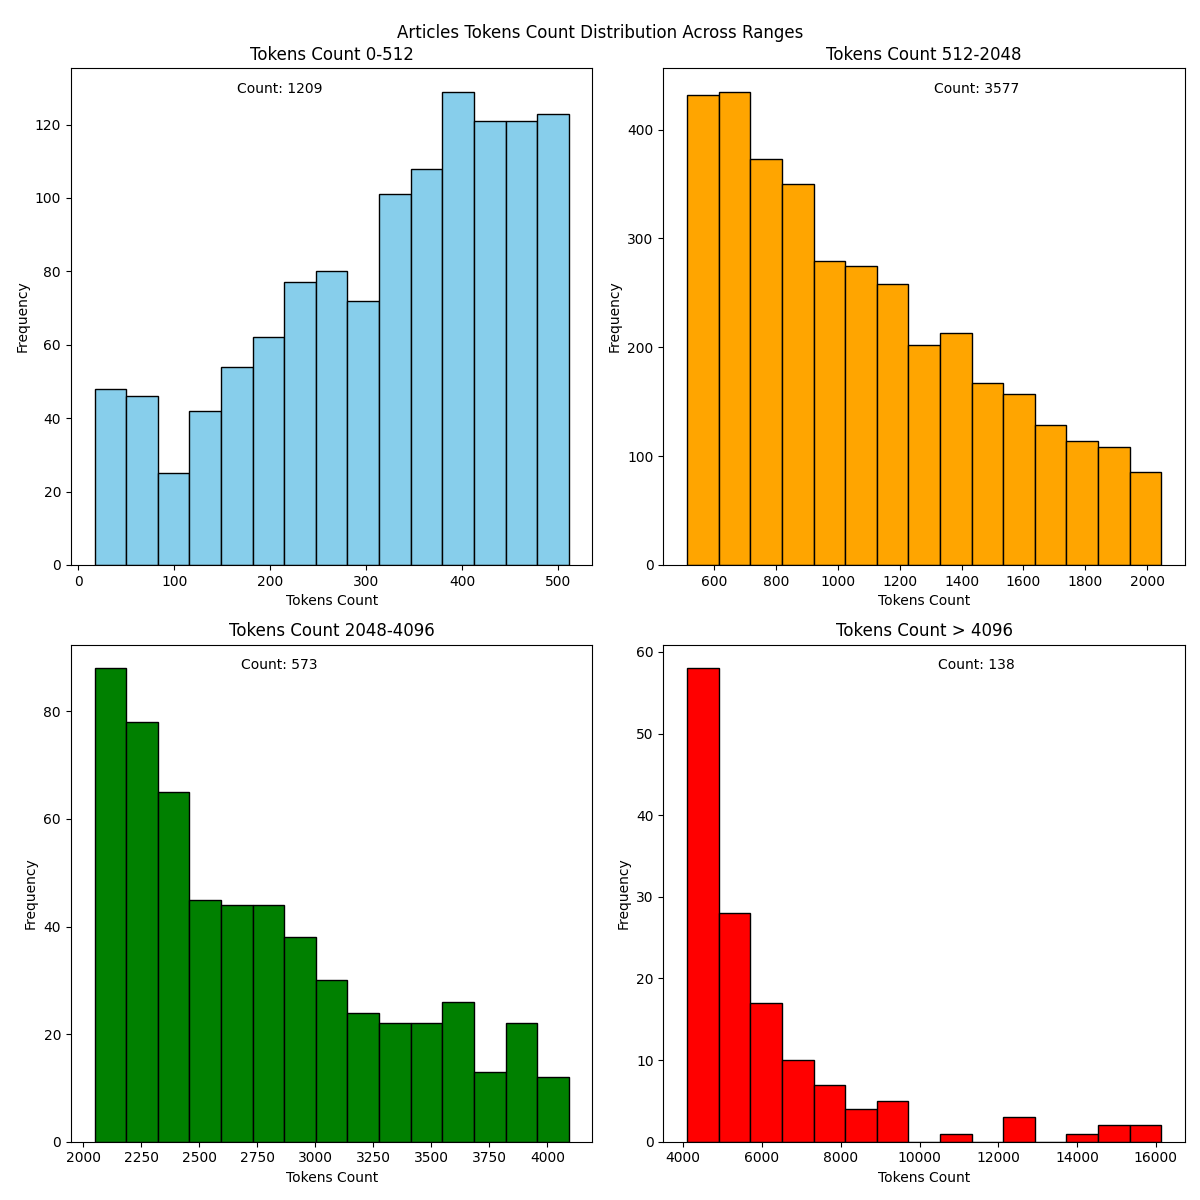
\includegraphics[width=0.9\linewidth]{figures/tokens_count_vx_split_hist.png}
    \caption{Articles tokens count distribution}
    \label{fig:tokens_hist_split}
\end{figure}

\begin{figure}[htbp]
    \centering
    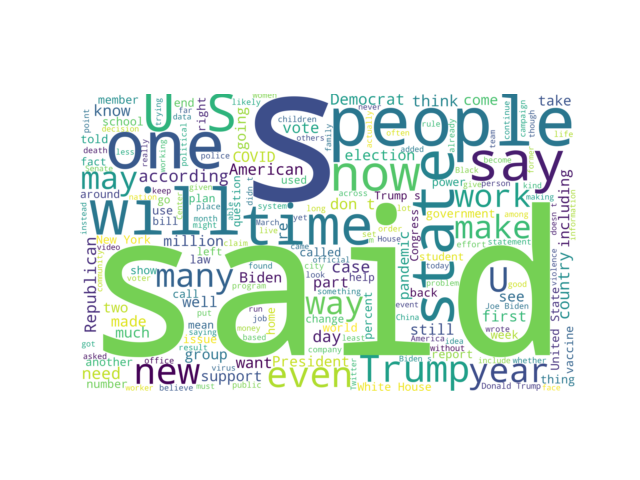
\includegraphics[width=0.7\linewidth]{figures/wordcloud_vx.png}
    \caption{Wordcloud}
    \label{fig:wordcloud}
\end{figure}




\begin{figure}[htbp]
    \centering
    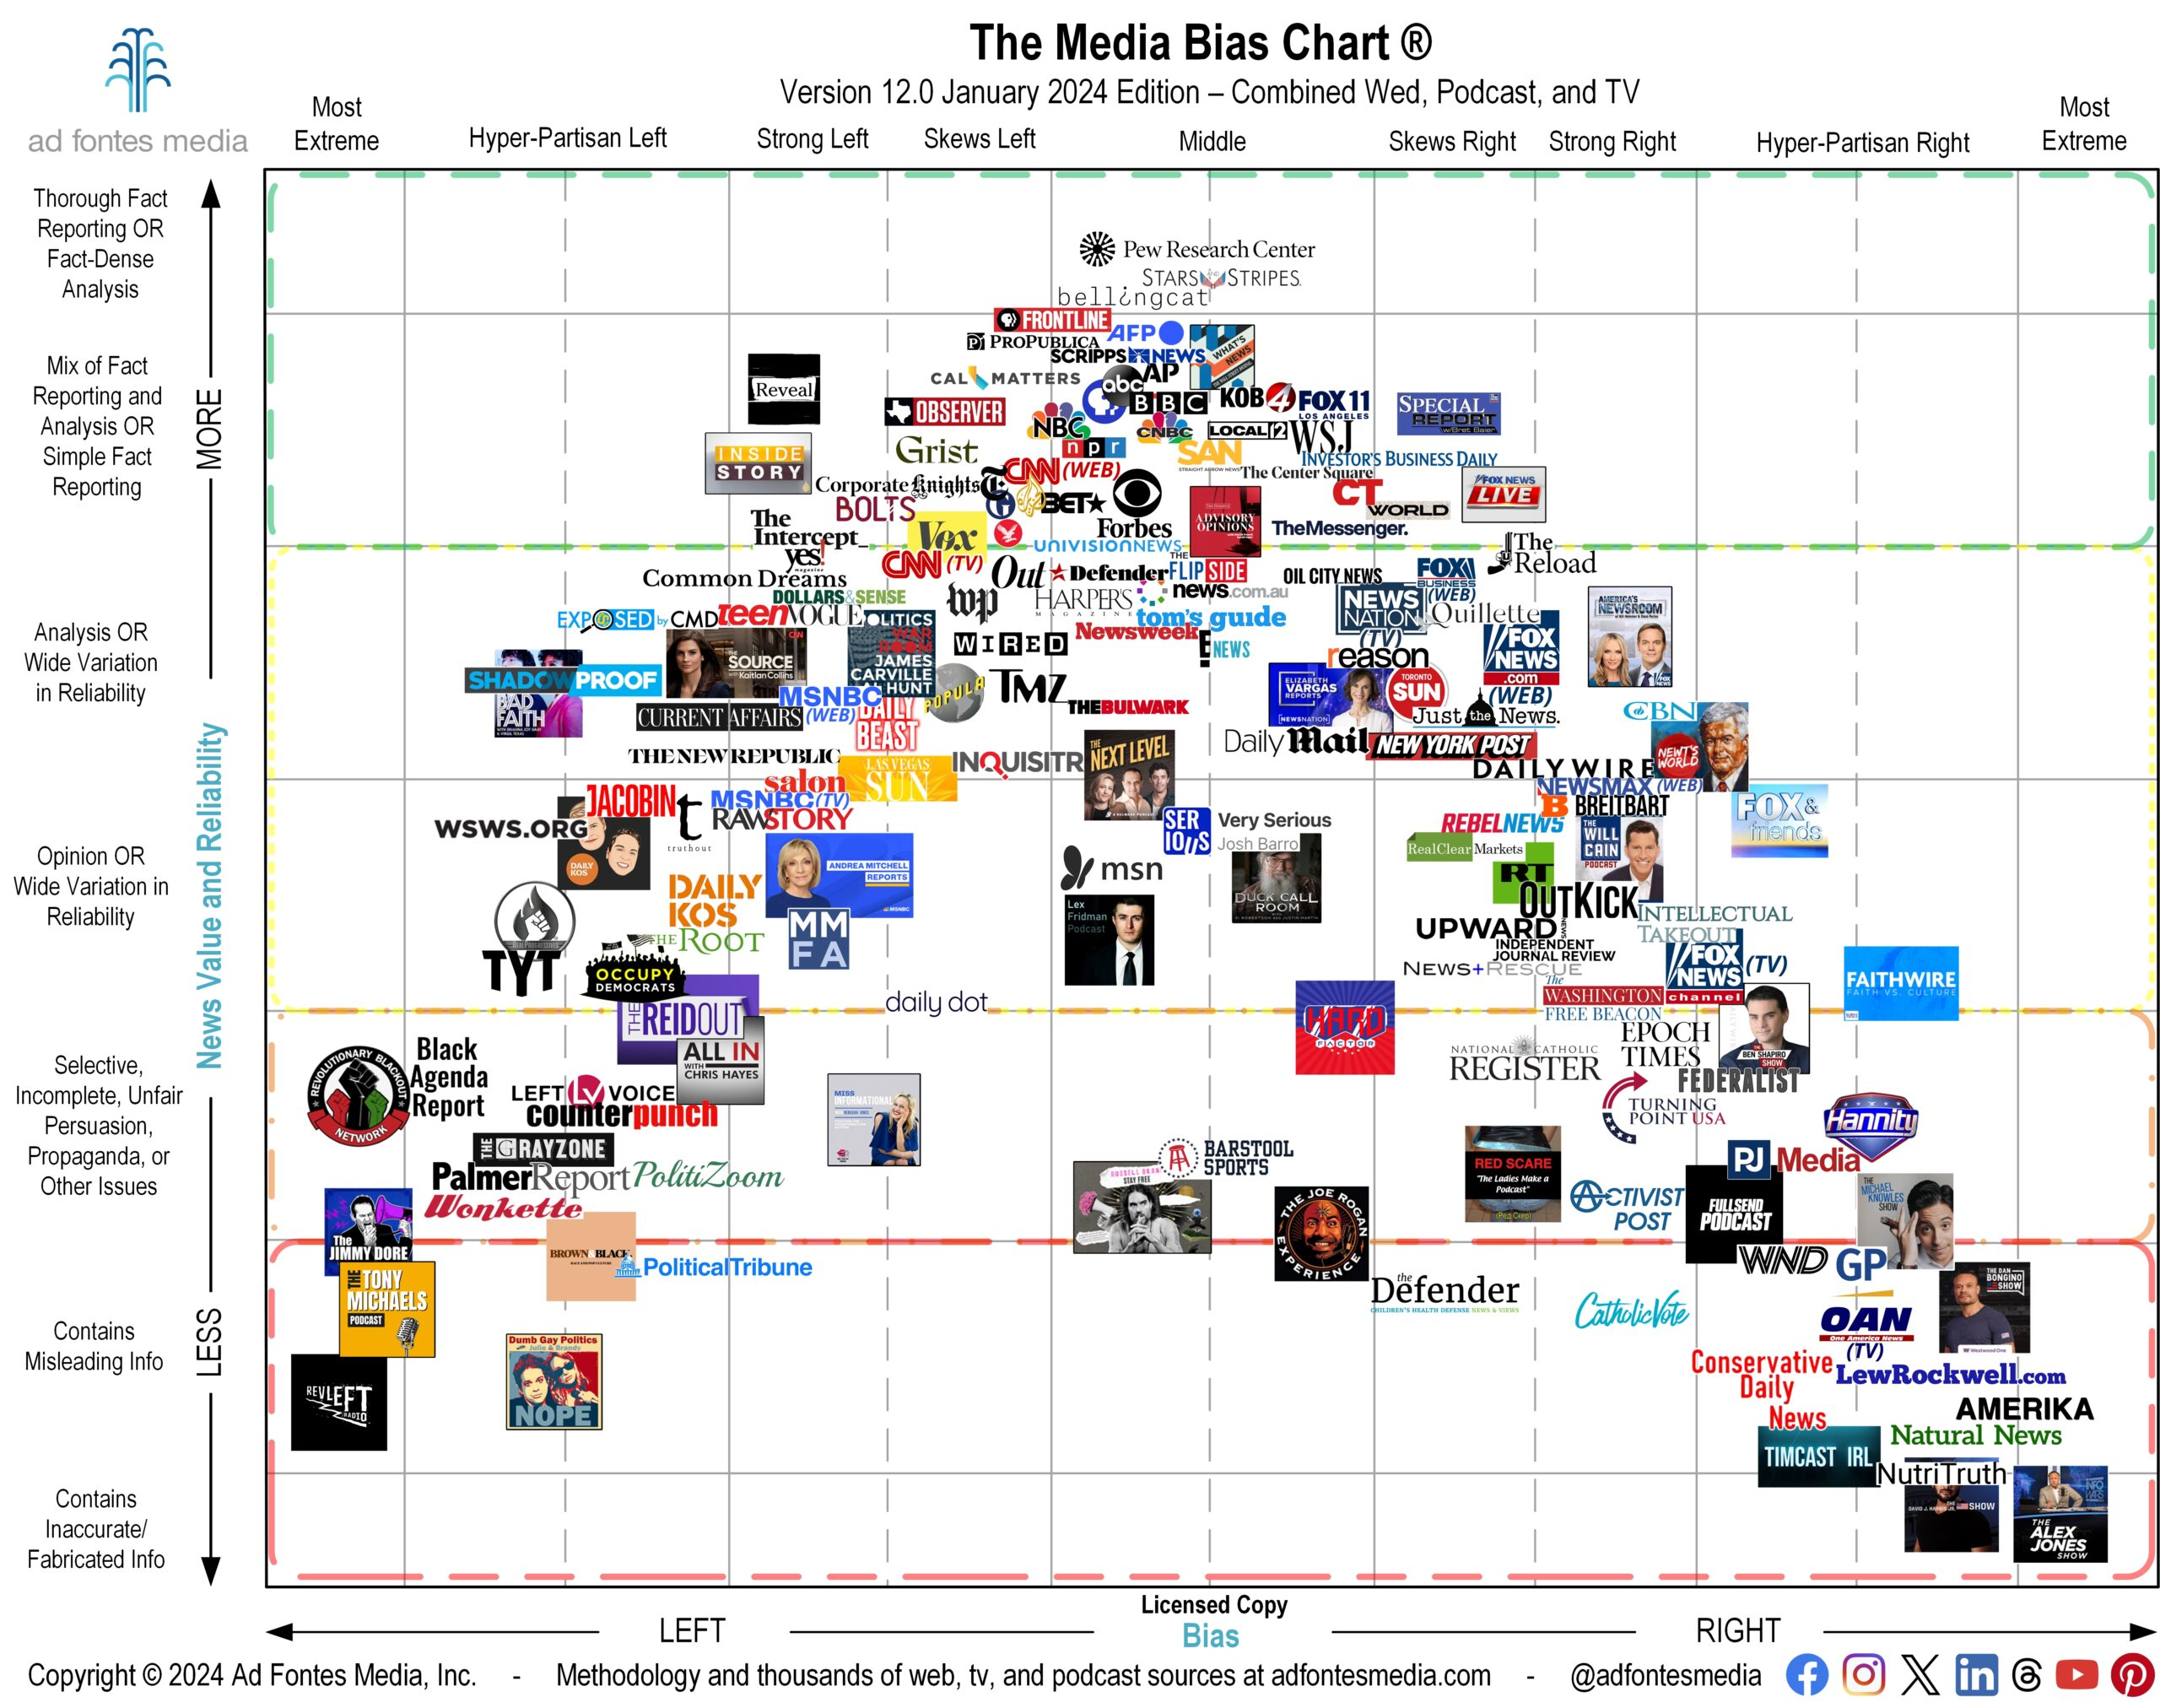
\includegraphics[width=0.8\linewidth]{images/Media-Bias-Chart-12.0_Jan-2024-Licensed-scaled.jpg}
    \caption{Ad Fontes media bias chart}
    \label{fig:adfontes-media-bias-chart}
\end{figure}

\begin{figure}[htbp]
    \centering
    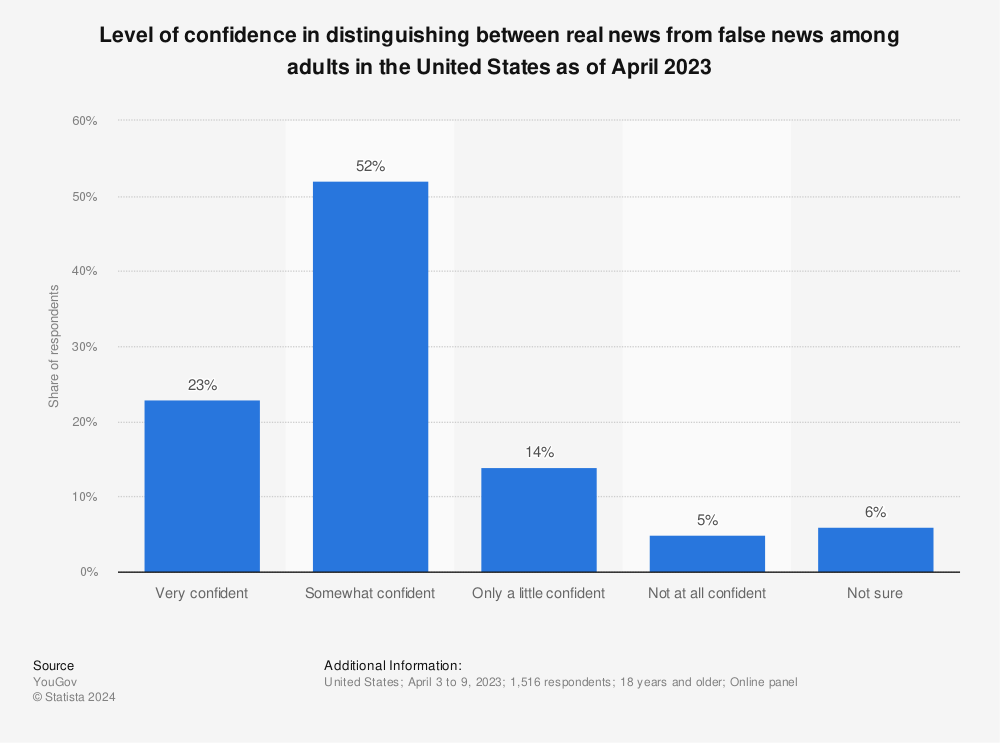
\includegraphics[width=0.9\linewidth]{images/statistic_id657090_ability-to-recognize-false-information-and-news-in-the-us-2023.png}
    \caption{Ability to recognise false information in the US \cite{yougov-2023-confidence}}
    \label{fig:ability-to-recognize-false-information-and-news-in-the-us-2023}
\end{figure}


\begin{algorithm}
    \begin{algorithmic}[1]
        \Procedure{FixWordsByDict}{content}
        \State $\text{words} \gets \text{Split content into list of words}$ \Comment{Using whitespace as delimiter}
        \State $\text{replaced\_words} \gets [\,]$
        \ForAll{$\text{word}$ \textbf{in} $\text{words}$}
        \State $\text{replaced\_word} \gets \text{WORD\_FIX\_DICT[word]}$ \Comment{Retrieve fixed word from dictionary}
        \If{$\text{replaced\_word}$ \textbf{is} $\text{None}$}
        \State $\text{replaced\_word} \gets \text{word}$ \Comment{Use original word if not found in dictionary}
        \EndIf
        \State $\text{replaced\_words.append(replaced\_word)}$
        \EndFor
        \State $\text{fixed\_content} \gets \text{Join replaced\_words into a single string with spaces}$
        \State \textbf{return} $\text{fixed\_content}$
        \EndProcedure
    \end{algorithmic}
    \caption{Fix word-level noise}
    \label{alg:word_level_noise_fix}
\end{algorithm}

\begin{algorithm}
    \begin{algorithmic}[1]
        \Procedure{RemoveNoisePhrases}{content}
        \State $\text{fixed\_content} \gets \text{content}$
        \ForAll{$(\text{word}, \text{fixed\_word})$ \textbf{in} $\text{PHRASE\_NOISE\_DICT}$}
        \State $\text{fixed\_content} \gets \text{fixed\_content.replace(word, fixed\_word)}$
        \EndFor
        \State \textbf{return} $\text{fixed\_content}$
        \EndProcedure
    \end{algorithmic}
    \caption{Remove phrase-level noise}
    \label{alg:phrase_level_noise_fix}
\end{algorithm}


%%% Local Variables: 
%%% mode: latex
%%% TeX-master: "thesis"
%%% End: 
